% Part A: DC sweep of Vin. VTC. Explain observations.

\FloatBarrier

\begin{figure}[h!]
	\centering
	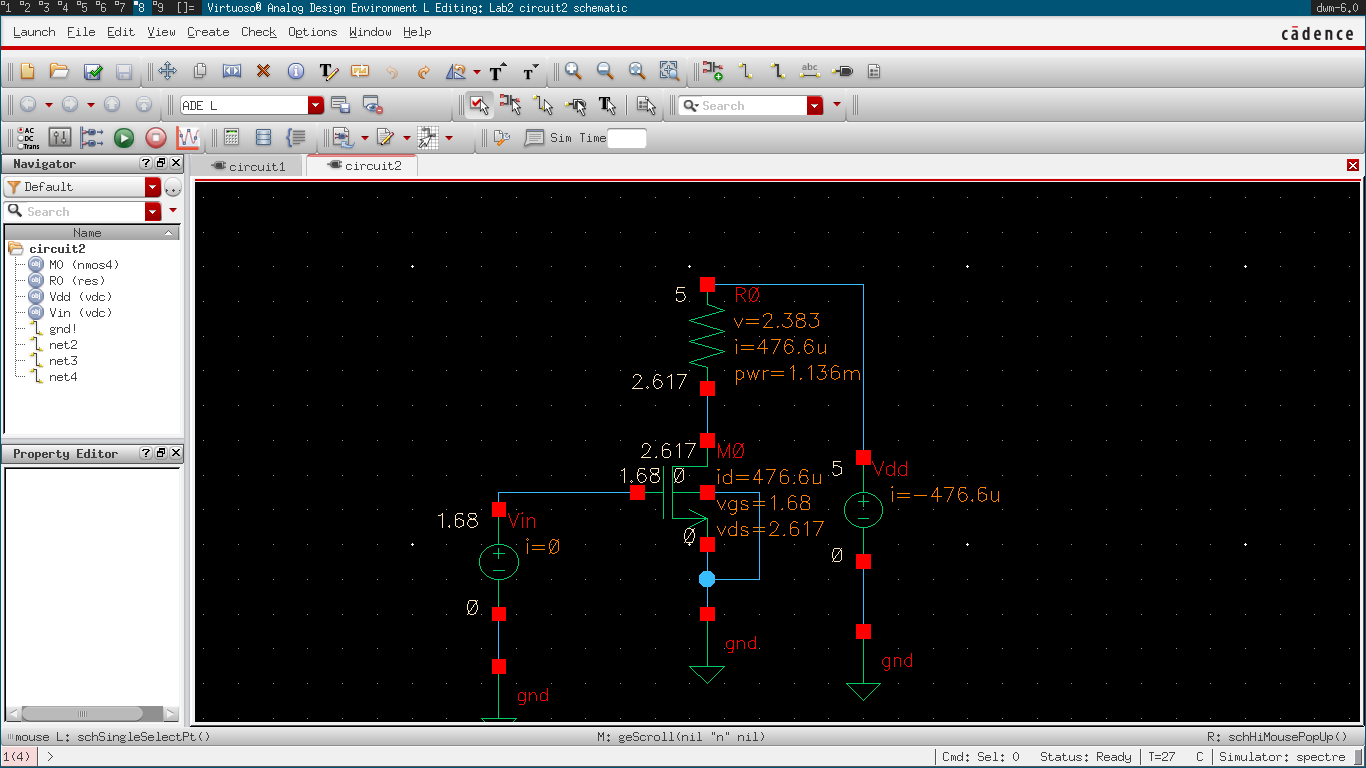
\includegraphics[scale=0.30]{./images/circuit2.PNG}
	\caption{Common-Source Amplifier}
	\label{fig:circuit2}
\end{figure}

\FloatBarrier

\FloatBarrier

\begin{figure}[h!]
	\centering
	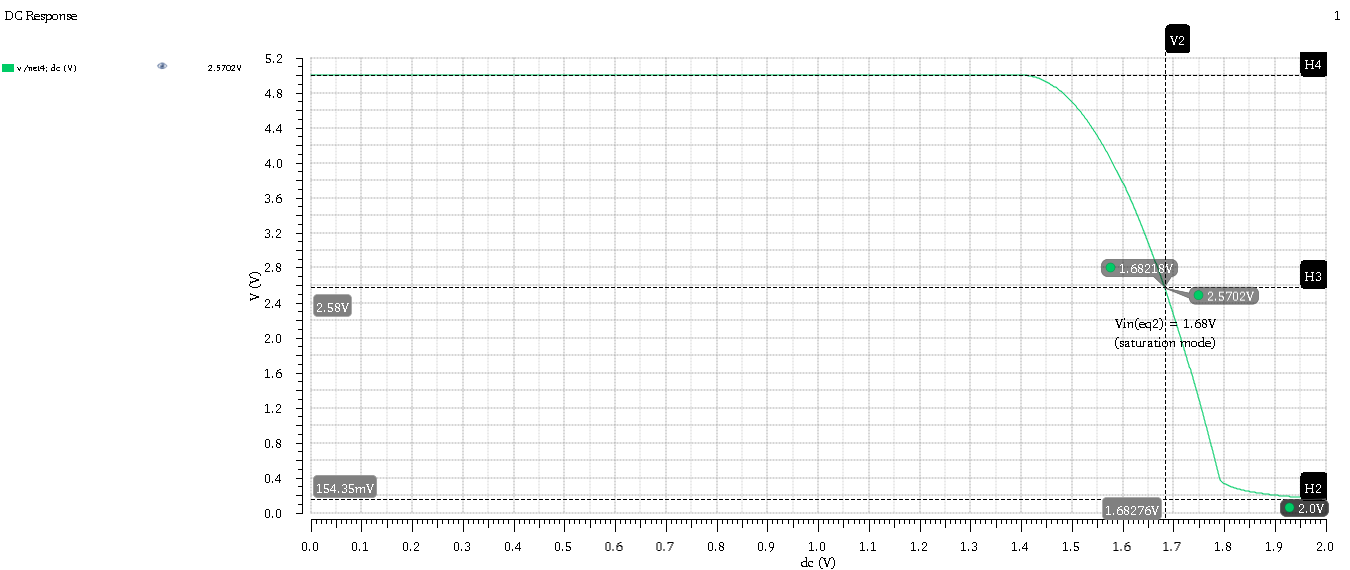
\includegraphics[scale=0.45]{./images/sim2_vtc.PNG}
	\caption{Voltage Transfer Characteristic for Common-Source Amplifier}
	\label{fig:sim2_vtc}
\end{figure}

\FloatBarrier
% Part B: Find V_in = V_ineq2
$V_{in(eq2)} = 1.68$\si{\volt} for this particular amplifier.
% In what region does the transistor operate?
The transistor operates in the saturation region at this point.
Common-source amplifiers start in cutoff mode for $V_{in}$ below the threshold voltage $V_{tn}$.
When $V_{in}$ is too large, they typically enter the triode mode.
For the region in between these two modes, the amplifier operates in saturation.
% DC op pt sim
Figure (\ref{fig:circuit2}) shows the results of a DC operating point simulation.
% Part C: Find gm and ro
These results can be used to calculate $g_{m}$ and $r_{o}$.

\FloatBarrier

\begin{table}[h!]
	\centering
	\caption{$g_{m}$ for Common-Source Amplifier}
	\label{tab:common_source_amp_gm}
	\csvautotabular{./tables/common_source_amp_gm.csv}
\end{table}

\FloatBarrier

\FloatBarrier

\begin{table}[h!]
	\centering
	\caption{$r_{o}$ for Common-Source Amplifier}
	\label{tab:common_source_amp_ro}
	\csvautotabular{./tables/common_source_amp_ro.csv}
\end{table}

\FloatBarrier

% Compare slope of Vout vs Vin at Vin,eq2 to result from equation

\FloatBarrier

\begin{figure}[h!]
	\centering
	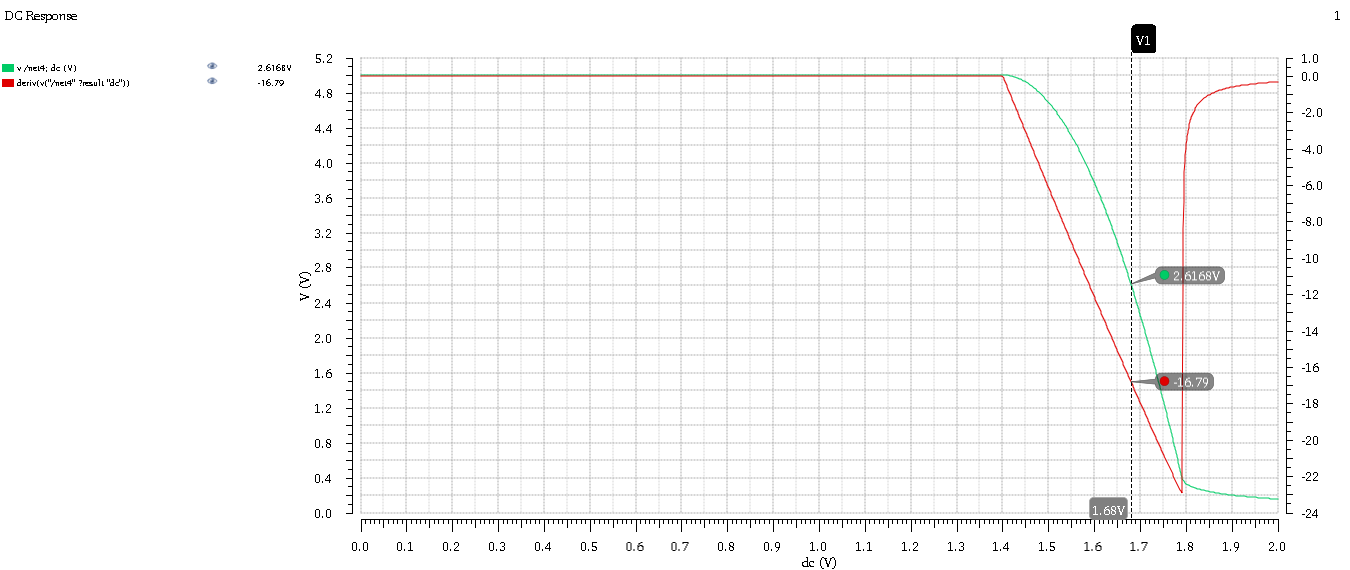
\includegraphics[scale=0.45]{./images/sim2_vtc_deriv.PNG}
	\caption{Common-Source Amplifier Voltage Transfer Characteristic with $\frac{dV_{out}}{dV_{in}}$ in Red}
	\label{fig:sim2_vtc_deriv}
\end{figure}

\FloatBarrier

At $V_{in(eq2)}$, the gain $\frac{dV_{out}}{dV_{in}}$ turns out to be about $-16.79$.
The gain can be calculated using the expression $A_{v} = -g_{m}(R_{D} || r_{o})$.

\FloatBarrier

\begin{table}[h!]
	\centering
	\caption{Common-Source Amplifier Gain}
	\label{tab:common_source_amp_gain}
	\csvautotabular{./tables/common_source_amp_gain_1.csv}
\end{table}

\FloatBarrier

% Compare DC and AC components of Vin and Vout for ss test

The small-signal behavior of the common-source amplifier is then analyzed.
A $1$\si{\milli\volt} amplitude, $1$\si{\mega\hertz} sine wave is applied at the gate when the transistor is biased at $V_{in(eq2)}$.

\FloatBarrier

\begin{figure}[h!]
	\centering
	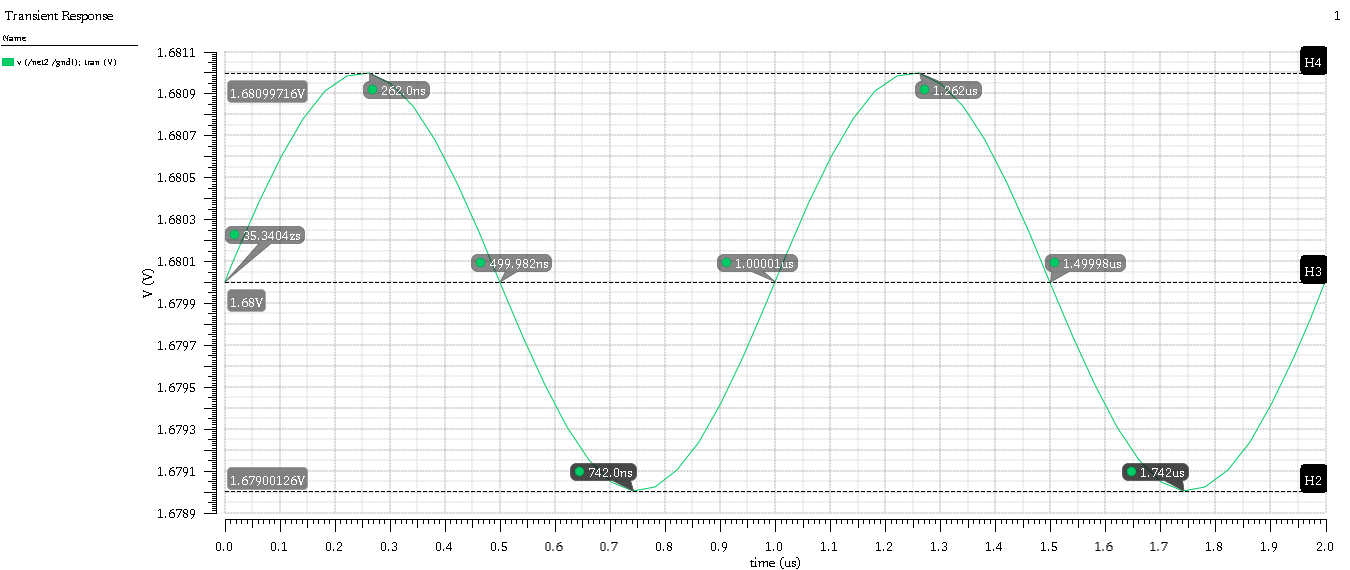
\includegraphics[scale=0.45]{./images/sim2_vin.PNG}
	\caption{$V_{in}$ Small-Signal Test of Common-Source Amplifier}
	\label{fig:sim2_vin}
\end{figure}

\FloatBarrier

\FloatBarrier

\begin{figure}[h!]
	\centering
	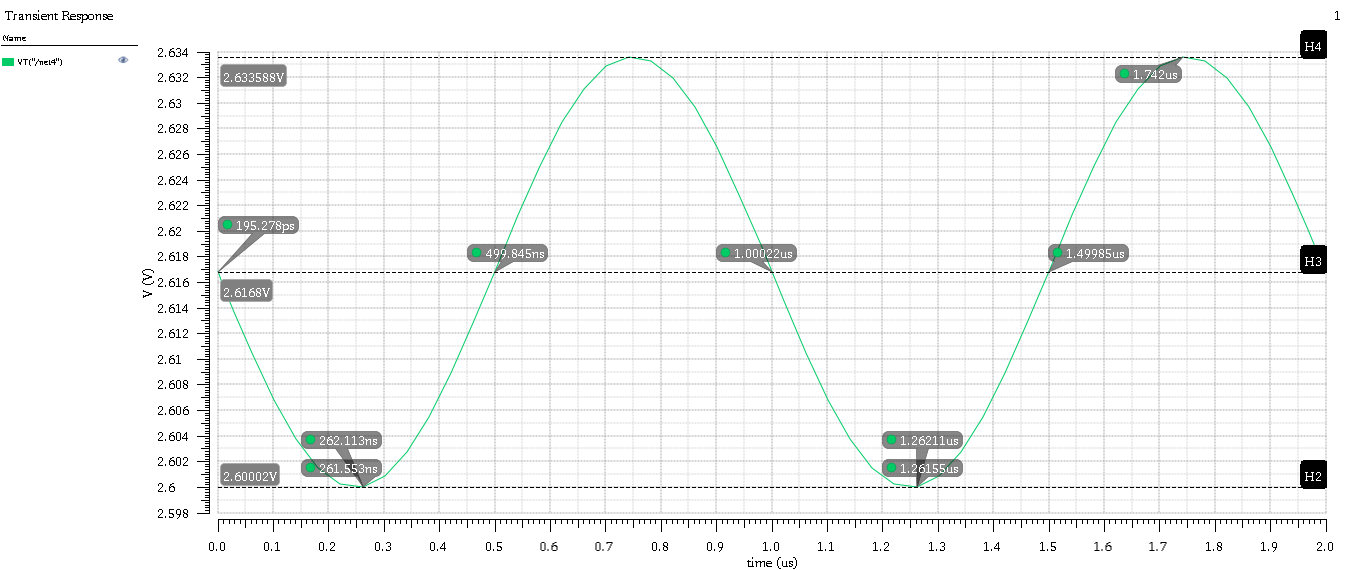
\includegraphics[scale=0.45]{./images/sim2_vout.PNG}
	\caption{$V_{out}$ Small-Signal Test of Common-Source Amplifier}
	\label{fig:sim2_vout}
\end{figure}

\FloatBarrier

The output signal is biased at the output voltage when $V_{in(eq2)}$ is applied at the gate of the transistor, whereas the input signal is biased at $V_{in(eq2)}$.
The ratio of the output signal's amplitude to the input signal's amplitude is about $16.8$, in line with the theoretical gain prediction and gain acquired from simulation plots.
The output signal is also out of phase by $180^{o}$, which is consistent with the fact that the gain is negative. \\

% Increase by 10mV. What changes?

The input bias is then increased by $10$\si{\milli\volt}.

\FloatBarrier

\begin{figure}[h!]
	\centering
	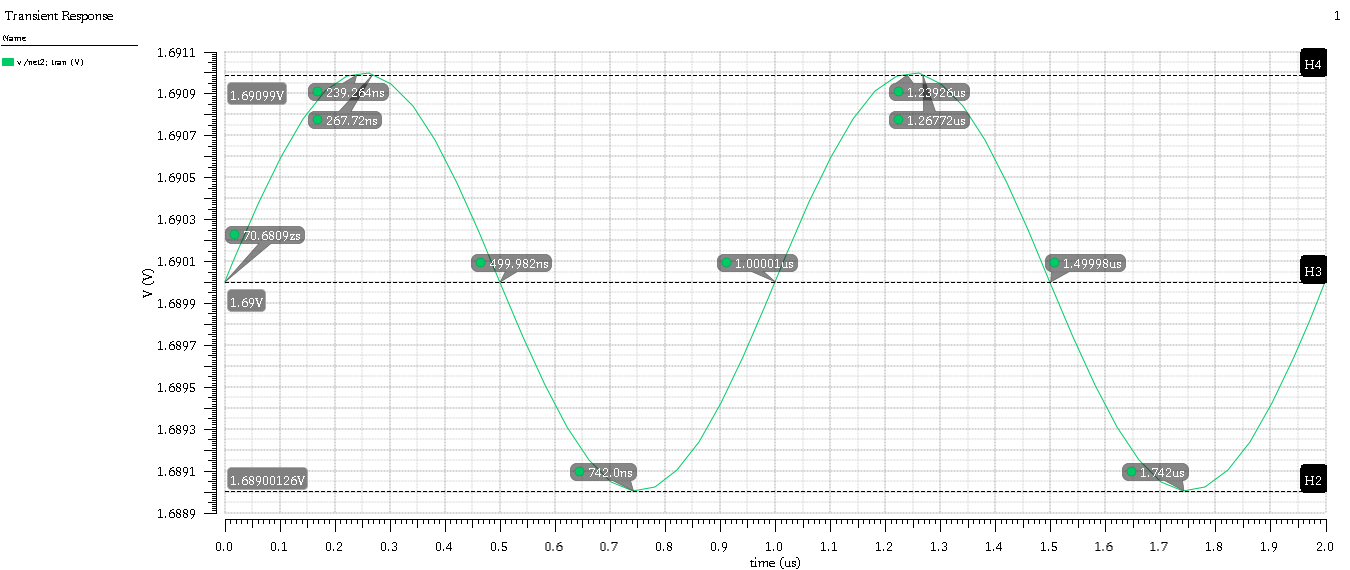
\includegraphics[scale=0.45]{./images/sim2_vin_plus10mV.PNG}
	\caption{$V_{in}$ for Small-Signal Test of Common-Source Amplifier after Increasing Input Bias by $10$\si{\milli\volt}}
	\label{fig:sim2_vin_plus10mV}
\end{figure}

\FloatBarrier

\FloatBarrier

\begin{figure}[h!]
	\centering
	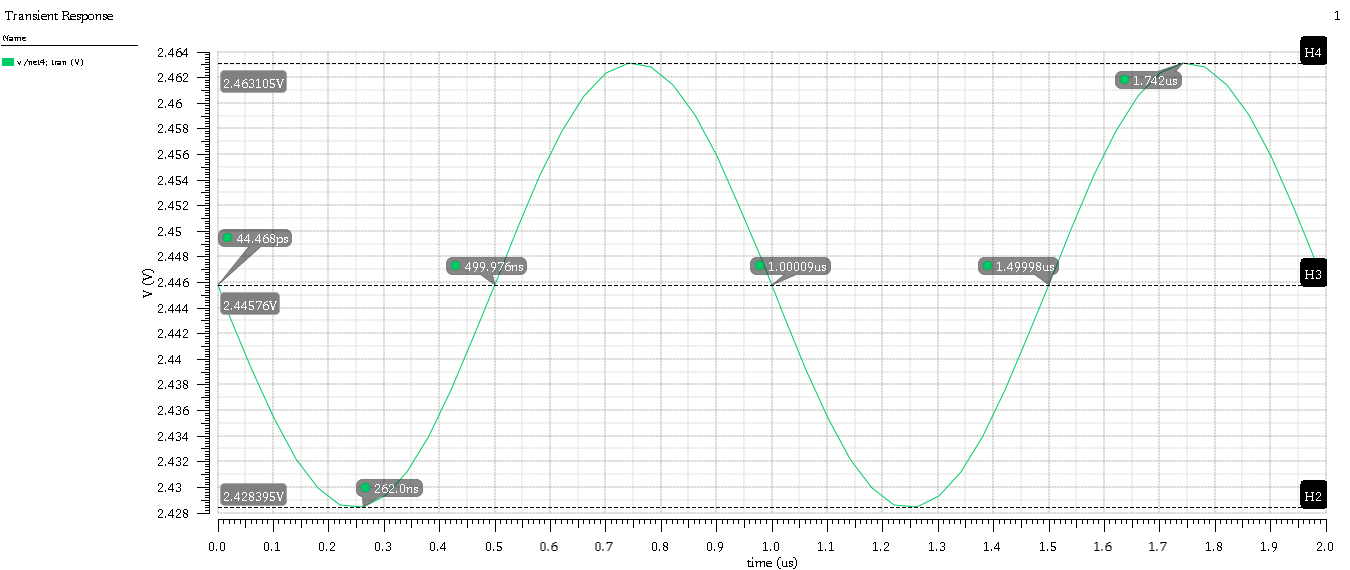
\includegraphics[scale=0.45]{./images/sim2_vout_plus10mV.PNG}
	\caption{$V_{out}$ for Small-Signal Test of Common-Source Amplifier after Increasing Input Bias by $10$\si{\milli\volt}}
	\label{fig:sim2_vout_plus10mV}
\end{figure}

\FloatBarrier

The output bias drops by roughly the gain of the amplifier times the change in the input bias $10$\si{\milli\volt}, precisely the behavior that is expected since the gain is directly related to the slope of the voltage transfer characteristic.
However, the gain appears to have increased in magnitude to about $-17.4$.
Thus, the gain of a common-source amplifier increases as the bias voltage is increased past the midpoint.
It should be noted that this is at the expense of output voltage swing.
